\documentclass[a4paper,fleqn]{cas-sc}

\usepackage[numbers]{natbib} \usepackage{graphicx} \usepackage{amsmath,amssymb} \usepackage{booktabs} \usepackage{url}

\begin{document} \let\WriteBookmarks\relax \def\floatpagepagefraction{1} \def\textpagefraction{.001}

\shorttitle{Uncertainty-Aware Multimodal Latent for Fetal Growth} \shortauthors{T. Cortinhal et al.}

\title[mode=title]{Screening recording errors in incomplete multimodal clinical records with a marginalising latent model}

\author[1]{Tiago Cortinhal}[orcid=0000-0002-8067-9521] \cormark[1] \ead{tiagofilipe.fernandes@usc.es}

\author[1,2]{C\'esar D\'iaz-Parga}

\author[3]{Gabriel Bernardino}

\author[1,2]{Marta Nu\~nez-Garcia}

\affiliation[1]{organization={Centro Singular de Investigaci\'on en Tecnolox\'ias Intelixentes (CiTIUS), Universidade de Santiago de Compostela}, city={Santiago de Compostela}, postcode={15782}, country={Spain}}

\affiliation[2]{organization={Departamento de Electr\'onica e Computaci\'on, Escola T\'ecnica Superior de Enxe\~nar\'ia, Universidade de Santiago de Compostela}, city={Santiago de Compostela}, postcode={15782}, country={Spain}}

\affiliation[3]{organization={BCN-MedTech, Universitat Pompeu Fabra}, city={Barcelona}, postcode={08018}, country={Spain}}

\cortext[1]{Corresponding author}

\begin{abstract}
\noindent\textbf{Objective:} Clinical registries assembled from routine examinations are structurally incomplete and contain recording errors. Using routine third-trimester fetal examinations (biometry, maternal, Doppler, and fetal-cardiac measurement blocks) we show that a latent model which \emph{marginalises} missing values, rather than imputing them, yields a reconstruction residual that serves as an automatic data-quality screen, and quantifies the uncertainty a record's incompleteness induces.
\noindent\textbf{Methods:} A linear-Gaussian factor model ($K=8$ by parallel analysis, VARIMAX-rotated) was fitted to $25$ measurements in four blocks from $977$ fetuses. The posterior precision sums contributions from observed measurements only, so no value is imputed. Each recorded value is screened by the standardised residual between the measurement and its reconstruction; the screen was evaluated on a synthetic benchmark with injected errors of known type ($6{,}000$ errors, $40{,}000$ clean records) and its flags verified against the source registry. Posterior calibration was assessed by censoring the Doppler block and scoring interval coverage on the held-out measurements.
\noindent\textbf{Results:} The residual flagged $38$ of $977$ records; $36$ were confirmed transcription errors in the source registry, all inconsistent within their own measurement block (e.g.\ an abdominal circumference of $35.6$\,cm reconstructed at $24.0$, registry value $23.6$). On the synthetic benchmark, sensitivity to cross-block inconsistencies increased from $0.09$ to $0.51$ as cross-block coupling increased, at fixed specificity. With the Doppler block censored, marginalised intervals covered held-out measurements in $97\%$ (nominal $95\%$) and $93\%$ (nominal $90\%$) of cases; multiple imputation by chained equations reached equal calibration only when given the same information, at the cost of a second modelling pipeline. The measurement blocks proved close to mutually uninformative (cross-block out-of-fold $R^2=0.023$), which localises what the screen can detect: within-block inconsistency on this cohort, cross-block inconsistency as coupling increases. The latent additionally orders fetuses along a continuous growth spectrum (Spearman $\rho = 0.55$ with birthweight centile) with no cluster structure, and its haemodynamic axis shows an association with adverse outcome among small-for-gestational-age fetuses, reported here as a secondary observation.
\noindent\textbf{Conclusion:} Marginalisation turns a standard factor model into a calibrated, assumption-light audit tool for incomplete multimodal registries: it abstains where data are absent, and its reconstruction residual finds the records that are wrong.
\end{abstract}

\begin{keywords}
data quality \sep error detection \sep missing data \sep latent-variable model \sep uncertainty quantification \sep multimodal clinical data \sep fetal growth
\end{keywords}

\maketitle



\section{Introduction}
Clinical registries assembled from routine care are the substrate of most retrospective medical machine learning, and they carry two defects that are usually handled separately: values that are \emph{absent}, because acquisition follows clinical discretion rather than a protocol, and values that are \emph{wrong}, introduced at transcription from source documents. The first is normally addressed by imputation, the second by manual audit or per-variable range checks. This paper shows that a single latent-variable model addresses both at once, provided missing values are marginalised rather than imputed.

Our test bed is a registry of routine third-trimester fetal examinations: $25$ measurements in four blocks --- fetal biometry, maternal characteristics, Doppler velocimetry, and fetal echocardiography --- from $977$ pregnancies. Doppler and cardiac panels are acquired at the discretion of the clinician, so entire blocks are absent by clinical decision rather than at random \cite{ref:littlerubin}, and the registry was populated by manual transcription. The cohort spans the full growth range ($169$ small-for-gestational-age newborns, of which $61$ severe; $77$ large-for-gestational-age), which matters because a data-quality screen must not mistake pathology for error.

Per-parameter range checks assess each value in isolation and cannot detect a value that is individually plausible but inconsistent with the rest of its record. Supervised error detectors require labelled errors, which registries do not have. Imputation-based pipelines fill the record before analysis, which conflates the two defects: an imputed value enters downstream analysis with the standing of a measurement, and an erroneous value that survives imputation contaminates the model fitted to it. What is needed is a representation that (i) accepts an arbitrary subset of observed measurements, (ii) reports how much the missing ones limit what it knows, and (iii) exposes, for every recorded value, how consistent that value is with the remainder of the record.

We show that a deliberately simple model --- a linear-Gaussian factor model whose posterior precision sums contributions from observed measurements only --- satisfies all three. Marginalisation makes the posterior width an honest function of what was acquired (a fetus without Doppler gets a wider posterior, not a filled-in guess), and the standardised residual between each measurement and its reconstruction is an automatic screen for recording errors that requires no computation beyond the model fit. On this registry the screen flagged $38$ of $977$ records, of which $36$ were confirmed transcription errors against the source documents; a synthetic benchmark with injected errors of known type characterises exactly when the screen can and cannot detect an error. The information structure of the data --- four blocks close to mutually uninformative --- turns out to determine both the screen's reach and the honest limits of any multimodal analysis of such records.

The contributions are: (1) a marginalising factor model as a data-quality instrument for incomplete multimodal registries, with its detection envelope characterised on a synthetic benchmark with injected errors of known type; (2) a registry-verified audit in which $36$ of $38$ flagged records were confirmed as transcription errors, all within-block, consistent with the measured information structure; (3) a calibration study under block censoring showing marginalisation matches multiple imputation without a second modelling pipeline; and (4) a characterisation of the latent representation itself --- continuous, not clustered --- with its clinical associations reported as secondary observations rather than claims.
\section{Related Work}

\noindent\textbf{Missing data in latent models.} Marginalizing missing entries out of a factor model is the standard likelihood treatment of missing data, known as full-information maximum likelihood \cite{ref:fiml} and computed by the expectation-maximization (EM) algorithm \cite{ref:em}. Multi-view Bayesian models such as MOFA and GFA handle entirely missing blocks in the same way \cite{ref:mofa,ref:gfa}, inferring a shared low-dimensional latent across several layers while accepting missing views and separating shared from view-specific factors.

\noindent\textbf{Missing modalities in clinical models.} Incomplete modalities are common in clinical data and are often handled by restricting the analysis to complete cases. Methods that explicitly accommodate missing modalities generally follow three strategies. The first trains models to tolerate missing modalities during learning \cite{ref:dropout}. The second designs architectures that operate on whichever modalities are available, for example through variable-sized inputs \cite{ref:hypermm} or adapted foundation models \cite{ref:mmdino}. The third modifies the fusion process itself, for example through confidence-guided staging \cite{ref:medpatch} or by disentangling shared and modality-specific representations \cite{ref:drfuse}.

\noindent\textbf{Uncertainty in multimodal models.} Calibrated uncertainty is usually learned, through deep ensembles, evidential heads, trusted multi-view fusion or conformal wrappers \cite{ref:sensoy,ref:han,ref:conformal}, and is often paired with selective prediction to abstain on low-confidence cases \cite{ref:selective}. A recent survey of missing-modality learning notes the lack of a principled framework for quantifying the contribution of individual modalities and the uncertainty induced by their absence \cite{ref:wu}.

\noindent\textbf{Automated data-quality screening.} Error detection in clinical registries is dominated by rule-based range and consistency checks, which assess each variable in isolation and require hand-written rules per variable. Learning-based approaches treat error detection as outlier detection in the population distribution, which conflates pathology with error in cohorts that span a wide clinical range. Reconstruction-based screening --- flagging values poorly predicted from the rest of their own record --- is standard in industrial anomaly detection but rarely applied to clinical registries, and to our knowledge has not previously been combined with a marginalising missing-data treatment, which is what allows the same fitted model to screen incomplete records without first imputing them.

\noindent\textbf{Fetal-growth characterization and imaging.} Latent-variable models have been developed to assess fetal size and Doppler flow. However, these models typically aim to identify discrete mixture classes \cite{ref:slaughter}. Data-driven phenotyping has successfully distinguished between severe and mild cases of fetal conditions \cite{ref:miranda}. Reviews indicate that the benefits of multimodal approaches are widespread, yet they are rarely subjected to significance testing \cite{ref:schouten}. Notably, the largest fetal growth imaging model \cite{ref:truong} outperforms the Hadlock formula, and learns from B-mode anatomical textures involving data from approximately 65,000 patients.

\section{Method} \begin{figure}[pos=t] \centering 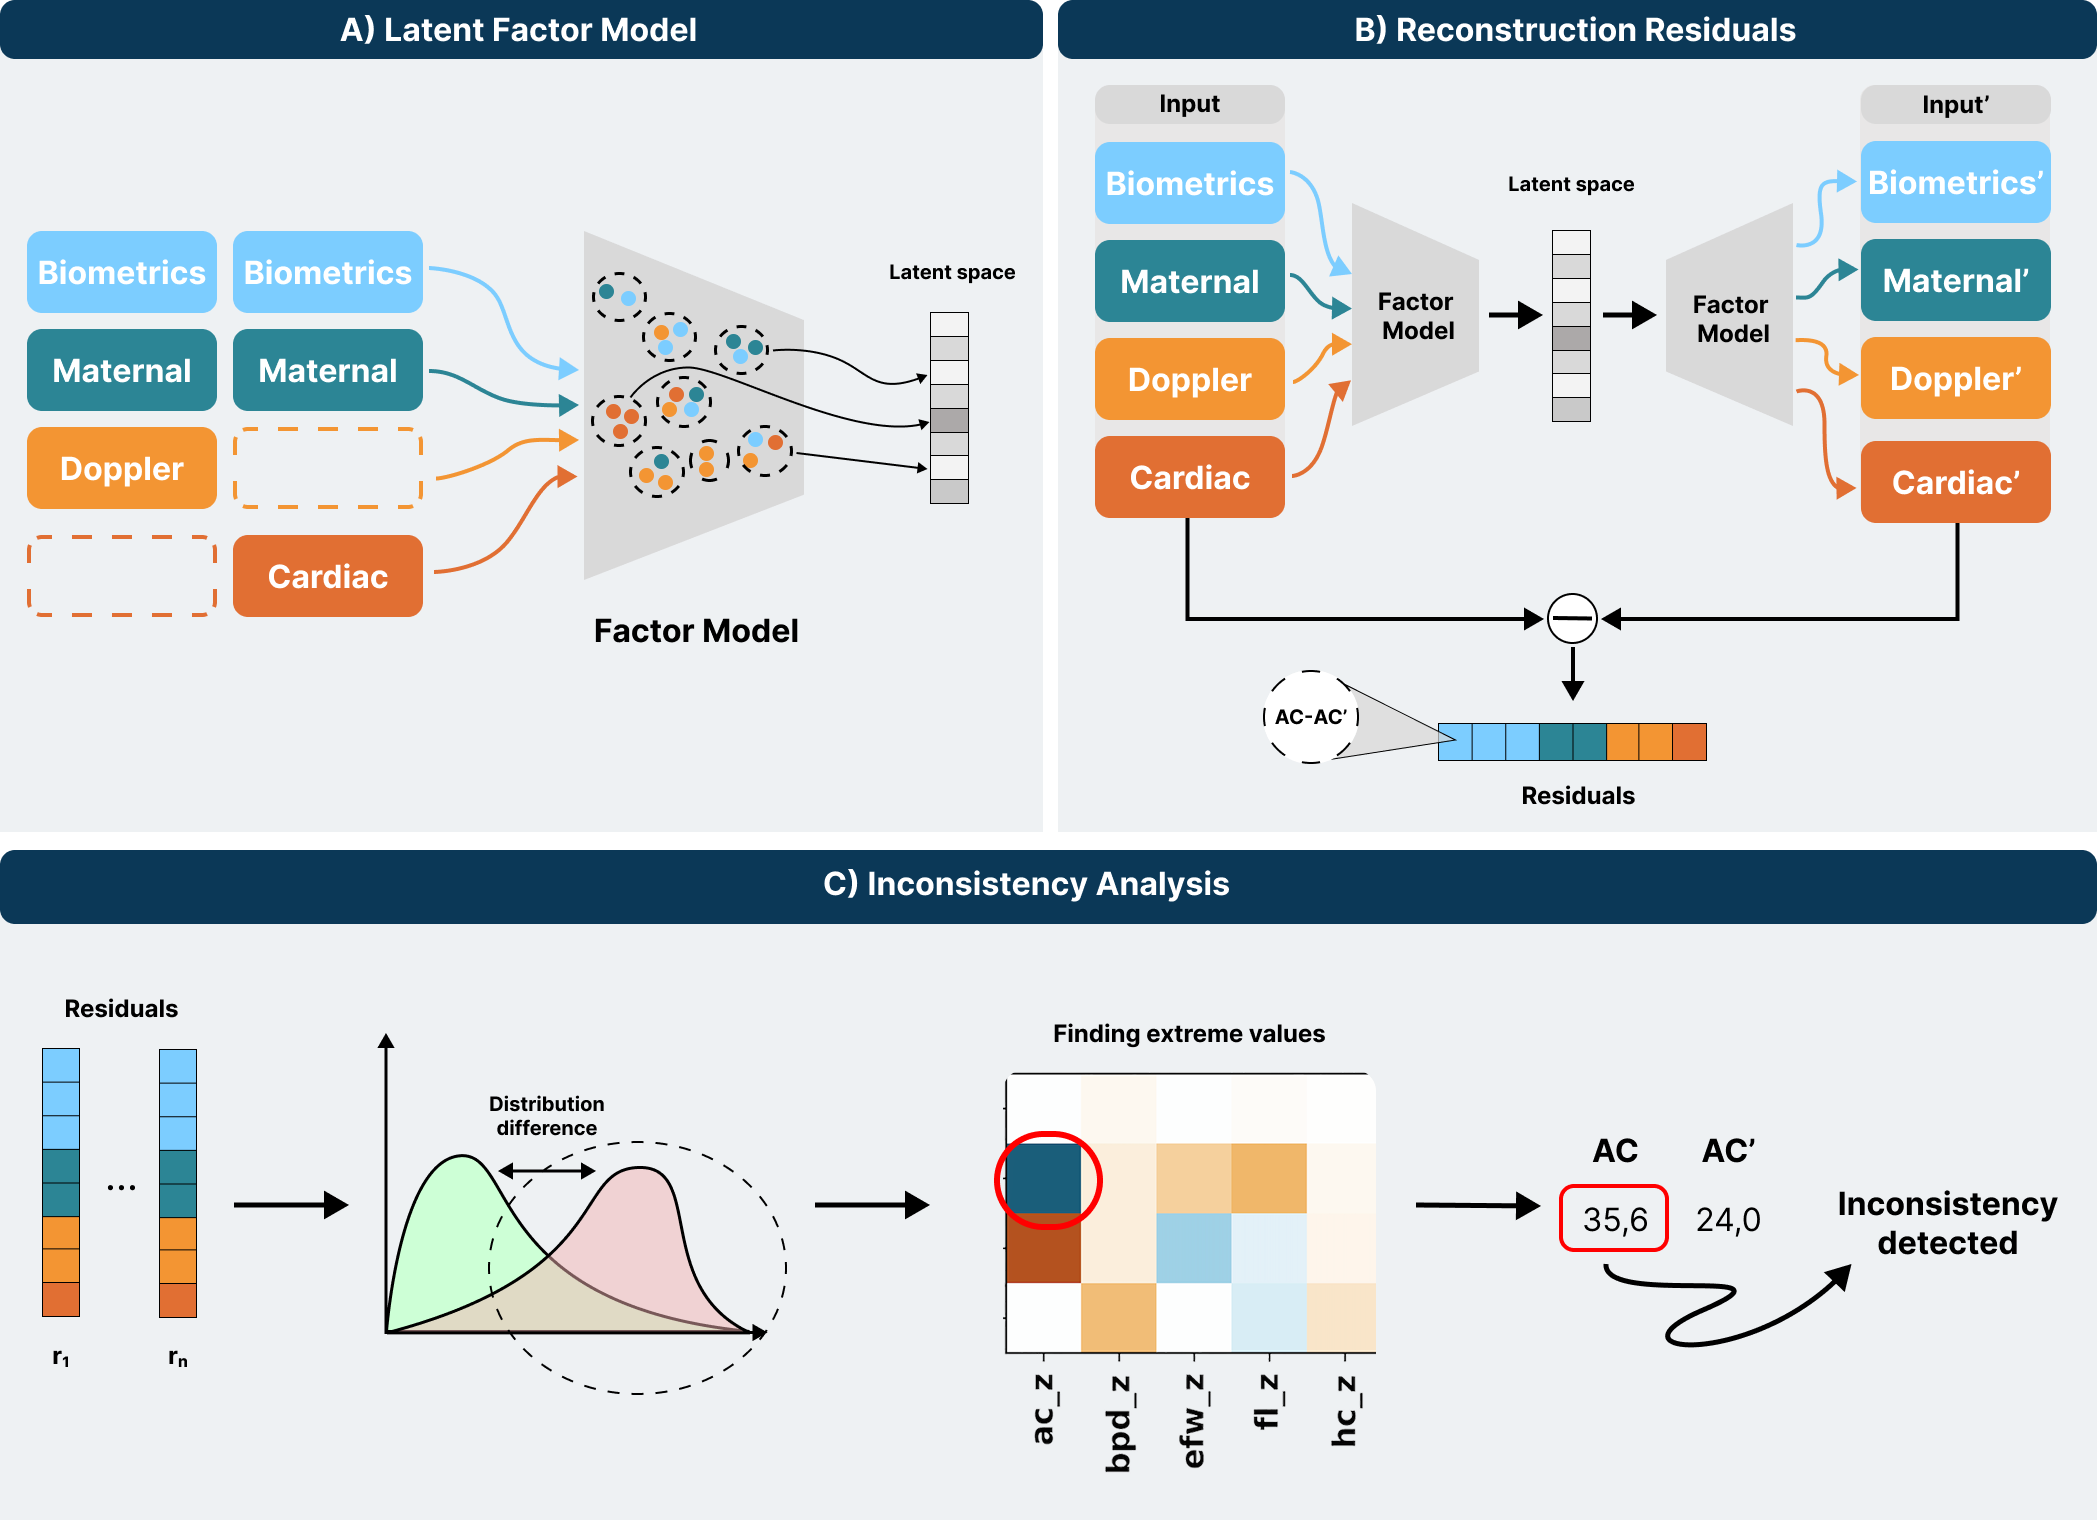
\includegraphics[width=\textwidth]{pipeline.png} \caption{Method overview, in three stages. \textbf{(a) Probabilistic generative model.} Two fetuses enter the factor model with different blocks available; the dashed empty boxes are blocks that were never acquired (cardiac for the first fetus, Doppler for the second). Each observed block contributes one precision term to the product-of-experts posterior (Eq.~\ref{eq:poe}); an absent block contributes no term and drops out of the sum, and nothing is imputed in its place. \textbf{(b) Reconstruction error analysis.} A fetus is passed forward to the latent space and back out to reconstructed blocks (primed), and the two are subtracted to give the standardised residual of Eq.~\ref{eq:resid}, one value per measurement. \textbf{(c) Inconsistency analysis.} Those residuals are compared against their cohort distribution to locate extreme entries. The worked example is an abdominal circumference recorded as $35.6$~cm where the latent reconstructs $24.0$~cm, which the screen flags.} \label{fig:pipeline} \end{figure}

\subsection{Cohort} We study a single-center cohort of $n=977$ fetuses with third-trimester ultrasound examinations. The factor model uses $25$ measurements, selected a priori to span four measurement blocks: fetal biometry, maternal characteristics, Doppler, and fetal-cardiac measurements. Variables were chosen to represent these clinical domains rather than for their association with the study outcomes, avoiding bias in the latent representation towards the labels used later for its interpretation.

The four blocks comprise (i) five fetal biometry z-scores referenced to the INTERGROWTH-21\textsuperscript{st} standard \cite{ref:ig21}, (ii) four maternal variables, (iii) five Doppler percentiles, and (iv) eleven fetal-cardiac percentiles.

The cohort spans the full growth continuum and includes $169$ SGA fetuses (of which $61$ are severe) and $77$ LGA fetuses. Outcomes independent of birthweight were available: preterm birth and admission to neonatal intensive care for 975 fetuses, and cord artery pH for 656.

Data incompleteness follows acquisition and is concentrated in the Doppler and fetal-cardiac blocks. Biometrics and maternal measurements are recorded for every fetus. A Doppler value is absent at a rate of $2.7\%$ and a fetal-cardiac value at $17.2\%$, therefore $11\%$ of records carry an incomplete Doppler panel and $70\%$ an incomplete cardiac panel, while a panel is absent in its entirety for $0.2\%$ and $0.7\%$ of records respectively.
%TODO CONFIRM MISSING RATES AND FULL MISSING RATES

\subsection{A missing-data factor model as a product of experts} The linear-Gaussian model assumes that the $25$ measurements of a fetus are generated by a small number of unobserved factors. Writing $\mathbf{x}_n\in\mathbb{R}^{25}$ for the measurement vector of fetus $n$ and $\mathbf{z}_n\in\mathbb{R}^{K}$ for its $K$ unobserved factor scores, the model is as following which we fit by expectation-maximization: \begin{equation} \mathbf{x}_n=\mathbf{W}\mathbf{z}_n+\boldsymbol{\mu}+\boldsymbol{\varepsilon}_n,\quad \mathbf{z}_n\sim\mathcal{N}(\mathbf{0},\mathbf{I}_K),\quad \boldsymbol{\varepsilon}_n\sim\mathcal{N}(\mathbf{0},\boldsymbol{\Psi}), \label{eq:fa} \end{equation} where $\mathbf{W}$ is a $25\times K$ matrix and it holds the factor loadings, which give the response of each measurement to each factor. $\boldsymbol{\mu}$ is a vector that holds the measurement means, and $\boldsymbol{\varepsilon}_n$ is measurement noise. The identity matrix $\mathbf{I}_K$ makes the factors a priori independent with unit variance. The noise covariance $\boldsymbol{\Psi}=\operatorname{diag}\boldsymbol{\psi}$ is diagonal, so its $j$-th entry $\psi_j$ is the variance of measurement $j$. We set K=8 using Horn's parallel analysis \cite{ref:stats}, which retains factors whose eigenvalues exceed those expected from random data of the same dimensions.

Imputing a Doppler panel that was never acquired treats estimated values as though they had been observed, placing the fetus with the same confidence as one with a complete examination. Instead marginalization leaves the posterior at its prior along the axes that otherwise would be constrained by the absent block. The posterior over the latent factors given only the observed measurements is Gaussian, with covariance $\mathbf{G}_n$ and mean $\mathbb{E}[\mathbf{z}_n]$:

\begin{equation}
    \mathbf{G}_n
    =
    \Bigl(\mathbf{I}_K
    +
    \textstyle\sum_{o(n)}
    \mathbf{W}_{m}^{\top}\boldsymbol{\Psi}_{m}^{-1}\mathbf{W}_{m}
    \Bigr)^{-1},
    \qquad
    \mathbb{E}[\mathbf{z}_n]
    =
    \mathbf{G}_n\,\mathbf{W}_{o}^{\top}\boldsymbol{\Psi}_{o}^{-1}
    (\mathbf{x}_{o}-\boldsymbol{\mu}_o).
    \label{eq:poe}
\end{equation}

where $m$ selects the rows belonging to one block, so $\mathbf{W}_{m}$ and $\boldsymbol{\Psi}_{m}$ are the loadings and noise variances, respectively, of that block's measurements alone, while $o$ selects everything observed for a given fetus.
The inverse of $\mathbf{G}_n$ is the posterior precision, and it is a sum of one term per observed block, as shown in Eq. \ref{eq:poe}. The model is a linear-Gaussian product of experts \cite{ref:poe}: each observed block contributes one precision term, the prior $\mathbf{I}_K$ contributes a further term, and a block that was not acquired contributes nothing to the sum. Because $\boldsymbol{\Psi}$ is diagonal, that sum decomposes further into one term $\mathbf{w}_j\mathbf{w}_j^{\top}/\psi_j$ for each observed measurement $j$. Fig.~\ref{fig:pipeline}a shows two fetuses missing different blocks, each placed from the terms available to it, with no value imputed for the absent one. As a result, the posterior widens only along the latent axes that the missing measurement block would have constrained. Figures~\ref{fig:pipeline}b–c follow this posterior through to the reconstruction residual described in Sect.~\ref{sec:trust}. For interpretability, we report factor loadings after a VARIMAX rotation \cite{ref:varimax}, which is an orthogonal rotation that maximizes the variance of the squared loadings within each factor, encouraging each measurement to load strongly on a single factor rather than several. The rotation changes only the reported basis of the latent subspace. The subspace itself, the fitted covariance, and all quantities derived from them remain unchanged.

\subsection{Posterior covariance and reconstruction residual}\label{sec:trust} The posterior covariance depends only on which blocks were observed (Eq.~\ref{eq:poe}) and not on their values, therefore two fetuses with the same observed blocks have the same covariance. Hence it does not account for a measurement that is present but implausible. To assess agreement between the observed measurements and the fitted model, we compute the mean standardized reconstruction residual: \begin{equation} \rho_n=\tfrac{1}{|o(n)|}\left\|\frac{\mathbf{x}_{n,o}-\mathbf{W}_o\,\mathbb{E}[\mathbf{z}_n]-\boldsymbol{\mu}_o}{\sqrt{\boldsymbol{\psi}_o}}\right\|^2 , \label{eq:resid} \end{equation} $\rho_n$ reports the agreement between the input and the fitted model. The numerator of Eq.\ref{eq:resid} is the raw residual between observed and reconstructed measurements. Dividing element-wise by $\sqrt{\boldsymbol{\psi}_o}$ standardizes each block by its noise level; while dividing by $|o(n)|$ normalizes for the number of observed blocks. A large $\rho_n$ flags poorly explained or anomalous cases.


\begin{figure}[pos=h] \centering 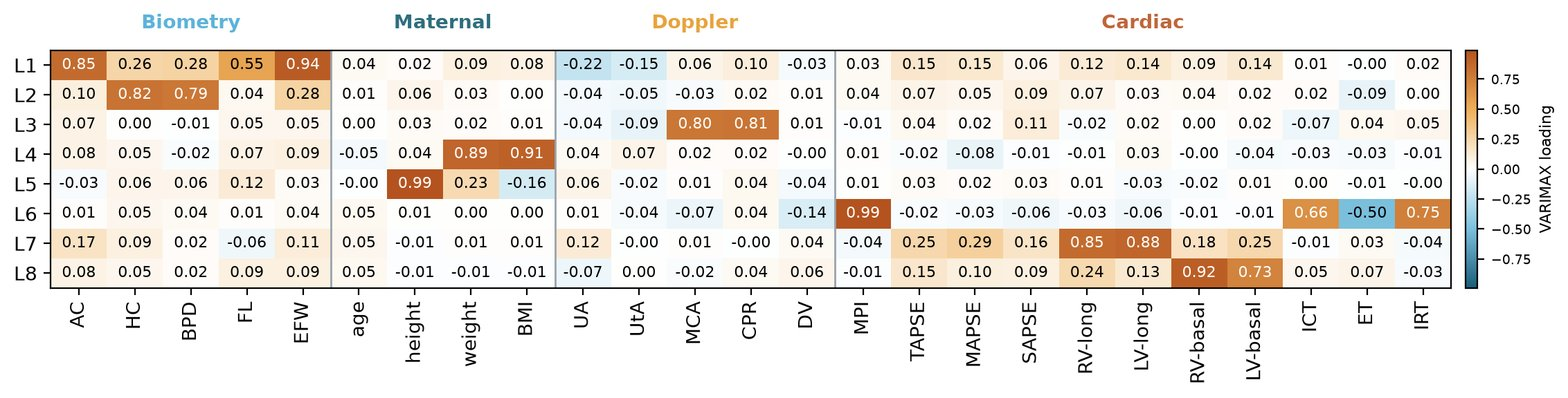
\includegraphics[width=1.0\textwidth]{loadings_heatmap_wide.jpg} \caption{VARIMAX loadings of the $K=8$ factor latent. Rows are the factors L1--L8, each named by its dominant block: fetal size (L1), head size (L2), haemodynamic redistribution from Doppler (L3), maternal body mass (L4), maternal stature (L5), and three cardiac axes (L6--L8). Color denotes the VARIMAX-rotated loading, with intensity reflecting the strength of the association between each measurement and latent factor.} \label{fig:heatmap} \end{figure}
   
\section{Experiments and Results} \subsection{Factor structure and block confinement}\label{sec:factors} The four measurement blocks carry little information about one another. Predicting each of the $25$
measurements from the measurements in other blocks gives an out-of-fold $R^2$ of $0.023$
($0.020$--$0.026$, $2.5$--$97.5$ percentile over $200$ independent five-fold splits). The same estimator
applied within a block recovers $0.509$ ($0.507$--$0.511$), so the near-zero cross-block value reflects the
data and not a failure of the predictor. The blocks differ: biometry is the most predictable from the others
($0.086$, $0.080$--$0.091$) and Doppler the least ($-0.015$, $-0.028$ to $-0.006$). Restricting to records
complete in every other block gives $-0.006$ ($-0.016$ to $0.004$) on a median of $277$ fetuses.

The latent space resolves into the 8 dimensions as portrayed in Fig.~\ref{fig:heatmap}. Two factors are biometric: L1 (EFW, AC, FL), which we call the size axis after its dominant loadings, and L2 (BPD, HC), the head axis. One is Doppler: L3 (MCA, CPR), the redistribution axis. Two are maternal: L4 (BMI, weight) and L5 (height). Three are cardiac: L6 (MPI, ICT, IRT, ET), myocardial function; L7 (LV-long, RV-long), ventricular long-axis function; and L8 (RV-basal, LV-basal), ventricular basal function.

The cardiac axis L6 is dominated by a derived measurement as it contains the myocardial performance index (MPI) alongside its components: $\mathrm{MPI}=(\mathrm{ICT}+\mathrm{IRT})/\mathrm{ET}$. 

To test whether block-aligned factors could arise from within-block structure alone, we refit the model on data in which the rows of each block were permuted independently, removing cross-block covariance while preserving each block's internal structure and missingness. Across $200$ refits the null gave a block purity of $0.992$ ($[0.987, 0.995]$), higher than the $0.962$ observed. Block alignment is therefore what this rotation produces by default and is not itself evidence of structure in the data; what distinguishes the fitted latent is the departure from that ceiling, consistent with cross-block loadings that independently permuted blocks do not generate and that a joint fit can represent.

Parallel analysis selected $K=8$, which was used throughout. The resulting latent factor structure was reproduced in all 24 random initializations and in $199$ of the $200$ bootstrap resamples.Nine rows show a graded association: the two Doppler indices that load the axis, uterine artery percentile,
gestational age at delivery, birthweight and its centile, SGA, severe SGA, and severe preeclampsia, which
falls from $11$ of $326$ in the lowest tertile to none in the highest. Maternal age, height, body mass
index, chronic hypertension, autoimmune disease and smoking show no gradient. Two rows reach $p<0.05$
without being graded: admission to intensive care ($8.9\%$, $0.6\%$, $2.5\%$) and corticosteroid
administration, both concentrated in the lowest tertile rather than increasing across tertiles. Cord artery
pH was recorded for $656$ fetuses; values below $7.10$ occurred in $14.2\%$, $6.0\%$ and $9.3\%$ of the
tertiles ($p=0.08$).



\subsection{Data consistency}\label{sec:consistency} A record is flagged when its squared standardized reconstruction error $|o(n)|\,\rho_n$ exceeds its $\chi^2$ reference with $|o(n)|-K$ degrees of freedom, with the false-discovery rate controlled at $5\%$ across the cohort. This flags $38$ of the $977$ records (Fig.~\ref{fig:pipeline}c). Checked against the source registry, $36$ are verifiable transcription errors. One fetus, for instance, is recorded with an abdominal circumference of $35.6$~cm where the registry gives $23.59$~cm. The remaining two are not errors but internally consistent outliers, such as a high body-mass index combined with short stature.

All $36$ confirmed errors are \emph{within-block}, in which the flagged value is inconsistent with the other measurements of its own block, as an abdominal circumference of $35.6$~cm is inconsistent with the head and femur measurements from the same examination. No confirmed cross-block errors occur in this cohort because the measurement blocks are nearly independent. Predicting any one block from the remaining three yields an out-of-fold $R^2_{\mathrm{cv}}=0.023$ ($0.020$--$0.026$), where the predictor is fitted on part of the cohort and scored on held-out records, so only $\approx4\%$ of the variance in one block is recoverable from the others.

All analyses reported before this subsection were performed after correcting these confirmed transcription errors and refitting the model. The residual analysis itself is computed on the original records, since its purpose is to identify those errors.

\subsection{Separating within- from cross-block detection}\label{sec:synth} The confirmed errors in our cohort are all within-block because the measurement blocks share little information ($R^2_{\mathrm{cv}}=0.023$; Sect.~\ref{sec:factors}). At this level of coupling, a value that is inconsistent only with measurements from other blocks is not expected to be detectable. To determine the level of cross-block dependence required for such inconsistencies to become detectable, we evaluated the reconstruction residual on synthetic data with controlled between-block coupling.

The synthetic panel follows the same linear-Gaussian model as the cohort, with the same 25 measurements arranged into the same four measurement blocks. A single parameter controls the amount of variance shared between blocks, producing the range of cross-block $R^2_{\mathrm{cv}}$ values in Table~\ref{tab:synth}. Errors are injected into measurements that are consistent within their own block but inconsistent with the remaining blocks, making them undetectable by construction using within-block information alone. We compare the reconstruction residual $\rho_n$ with a marginal z-score, a within-block predictor, and the Mahalanobis distance.

Table~\ref{tab:synth} shows that the sensitivity of $\rho_n$ increases monotonically from 0.094 to 0.514 as cross-block coupling increases. In contrast, the within-block comparator never exceeds 0.077, confirming that the injected errors cannot be detected using information confined to a single block. The Mahalanobis distance performs similarly to $\rho_n$ at low coupling but becomes progressively less sensitive as coupling increases.

Cross-block detection becomes appreciable above $R^2_{\mathrm{cv}}\approx0.13$. Because our cohort lies at $R^2_{\mathrm{cv}}=0.023$, the absence of confirmed cross-block errors is expected rather than a limitation of the reconstruction residual.

\begin{table}[width=\linewidth,cols=7,pos=h] \centering

\small \begin{tabular}{lcccccc} \toprule cross-block $R^2_{\mathrm{cv}}$ & $0.00$ & $0.13$ & $0.32$ & $0.47$ & $0.57$ & $0.66$ \\ \midrule per-variable $|z|$ & 0.045 & 0.045 & 0.045 & 0.043 & 0.046 & 0.045 \\ within-block control & 0.077 & 0.058 & 0.039 & 0.036 & 0.037 & 0.040 \\ reconstruction residual $\rho_n$ & \textbf{0.094} & 0.123 & \textbf{0.226} & \textbf{0.336} & \textbf{0.416} & \textbf{0.514} \\ Mahalanobis comparator & 0.090 & \textbf{0.126} & 0.217 & 0.311 & 0.381 & 0.470 \\ \bottomrule \end{tabular} 
\caption{Synthetic benchmark for detecting injected cross-block inconsistencies. Entries report the fraction of injected errors detected at a nominal $5\%$ false-positive rate as cross-block coupling ($R^2_{\mathrm{cv}}$) increases. Results are shown for the reconstruction residual $\rho_n$, a per-variable marginal z-score, a within-block predictor, and the Mahalanobis distance. Each cell is estimated from 6,000 injected errors and 40,000 clean records using the value of K selected by parallel analysis. Detection thresholds are calibrated separately for each number of observed measurements; achieved false-positive rates ranged from $0.048$ to $0.066$ (mean $0.053$).  }
\label{tab:synth} 
\end{table}

\noindent\textbf{Code and data availability.} The model, the residual screen and the synthetic benchmark are released at \url{https://github.com/TiagoCortinhal/fgr-geometry}. The synthetic benchmark is self-contained and reproduces Table~\ref{tab:synth} without access to the private cohort. The clinical tables cannot be shared.

\subsection{Uncertainty under incomplete acquisition} The trace of the posterior covariance decreases monotonically with the number of observed measurements ($\rho=-0.98$). Because the covariance is defined per latent axis, each fetus is represented by a region whose width differs from one axis to another. Figure~\ref{fig:uncert} shows these regions on L1 and L3. A fetus with the full panel is a compact region. Censoring its Doppler block widens the posterior along L3 while leaving its extent on L1 unchanged, whereas incomplete biometry widens the posterior along L1 instead. L1 remains narrow for every fetus (SD $0.20$), reflecting the near-complete availability of biometric measurements. By contrast, L3 is wider ($0.37$) and approaches its prior width ($0.98$) when no Doppler information was available. Consequently, the redistribution axis is informative only for the $89\%$ of fetuses ($93\%$ of the SGA fetuses) with a complete Doppler panel.

To validate these uncertainty estimates against observed data rather than the model's own latent
representation, we censored the Doppler block and tested whether the resulting predictive intervals covered
the held-out measurements. Censoring was applied in five folds, and both the factor model and the
comparator below were fitted on the censored matrix only, so neither had access to the values it was asked
to cover. Marginalisation covered $0.974$ of the $4{,}350$ held-out measurements at the nominal $95\%$
level and $0.925$ at the $90\%$ level. Multiple imputation by chained equations ($20$ draws, interval from
the between-draw variance) covered $0.954$ and $0.890$ on the same measurements, with a mean interval width
of $0.980$ against $0.979$ for marginalisation. Single-value imputation returns no interval. Unlike the reconstruction residual $\rho_n$, which depends on the observed values, the posterior width depends only on which measurements were acquired.

Near-independent blocks raise the question of whether a joint model is required at all. Hiding
$15\%$ of observed cells at random and reconstructing them, the joint eight-factor model gives a held-out
mean squared error of $0.589\pm0.010$ over five repeats, against $0.626\pm0.012$ for four per-block models
of matched total latent dimension. The joint fit is lower by more than twice the spread of either.

\begin{figure}[pos=h] \centering 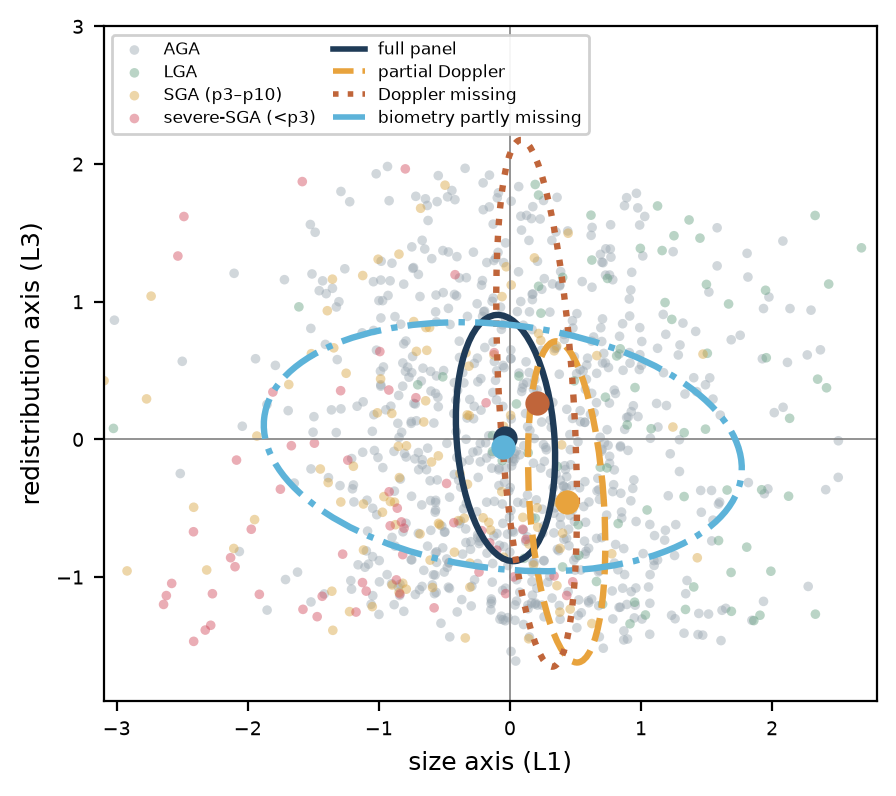
\includegraphics[width=0.80\textwidth]{uncertainty_region.png} \caption{Modality-conditional uncertainty on the fetal size (L1) and redistribution (L3) axes. Each fetus is a region whose shape follows which blocks were measured: a full panel is narrow, hiding the Doppler block widens the region along the redistribution axis, and incomplete biometry widens it along L1. Points are coloured by outcome.} \label{fig:uncert} \end{figure}

\subsection{Structure of the latent representation} The latent representation is organised around a continuous growth spectrum. Position along L1, the fetal size axis, correlates with birthweight centile (Spearman $\rho=0.55$, $p<0.001$), and SGA and LGA occupy near-opposite directions in the latent space (cosine -0.87; SGA against LGA, -0.96). Alignment is reported throughout as the cosine of the angle between two directions in the latent space, where 1 denotes coincidence, 0 orthogonality, and -1 opposite directions.

Three statistics agree that the space is unimodal rather than clustered. Hartigan's dip statistic measures the largest departure of a distribution from the closest unimodal one; here $p=0.99$ \cite{ref:dip}, so the scores are as compatible with a single mode as a unimodal distribution itself would be. The gap statistic compares within-cluster dispersion at each candidate number of clusters against the dispersion expected under a uniform reference distribution, and selects one cluster \cite{ref:gap}. The silhouette coefficient, which for each fetus compares its distance to its own cluster against its distance to the nearest other cluster and runs from $-1$ to $+1$, is $0.07$ at three clusters, close to the zero expected when a partition is arbitrary. Together, these results indicate that the latent representation forms a continuous growth spectrum rather than partitioning fetuses into discrete phenotypes.

This continuous structure is illustrated Fig.~\ref{fig:groups}. Fetuses are plotted on L1, the axis with the largest association with birthweight centile, and on L3, the haemodynamic redistribution axis. The three birthweight groups occupy overlapping regions of one gradient with no boundary between them, and the severe-SGA cases fall within the range of the SGA cases rather than forming a separate group at the low-size extreme.

Severe SGA cases are not separated from SGA along the fetal size axis, but they are shifted along the haemodynamic redistribution axis, with a mean L3 coordinate of $-0.55$ compared with $+0.05$ in AGA fetuses. L3 loads on the cerebroplacental ratio (CPR) ($+0.81$) and middle cerebral artery (MCA) percentile ($+0.80$), with no other loading exceeding $0.15$, indicating that low L3 scores correspond to reduced CPR and MCA. This interpretation is supported by the measured Doppler values, where severe SGA fetuses have a mean MCA percentile of $32$ versus $48$ in AGA, and a mean CPR percentile of $2$4 versus $44$.

\begin{figure}[pos=h] \centering 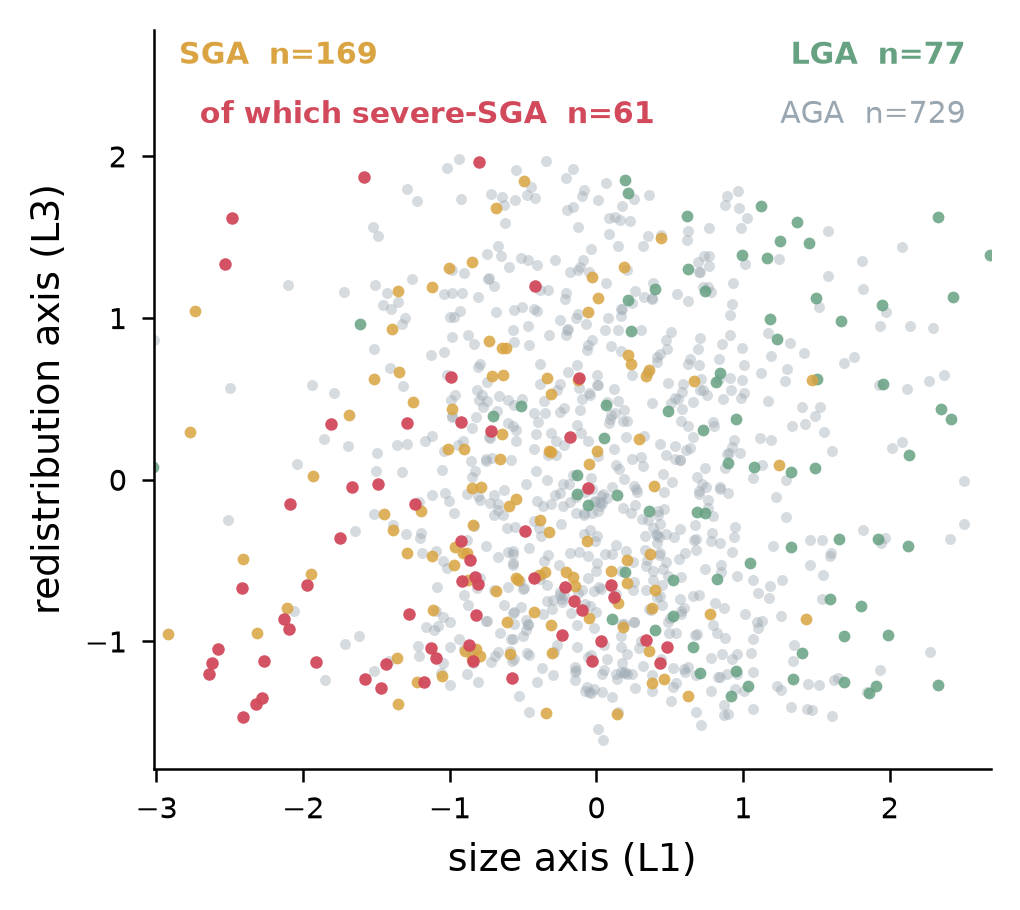
\includegraphics[width=0.72\linewidth]{fig3.png} \caption{Birthweight-defined growth groups in the latent space, on the axis carrying the largest association with birthweight centile (L1) and the axis carrying the largest size-independent association (L3). The groups occupy overlapping regions of a continuous gradient rather than separate clusters, and severe-SGA cases lie within the SGA range rather than apart from it.} \label{fig:groups} \end{figure}

\subsection{Secondary observation: outcome association among small-for-gestational-age fetuses}
\label{sec:checks}
The registry records two outcomes not defined by birthweight: preterm birth and neonatal intensive-care admission ($975$ of $977$ fetuses; composite events in $71$, including $25$ of $169$ SGA). We report the association as a secondary observation on the representation rather than a clinical claim. Among SGA fetuses, the haemodynamic redistribution axis separated adverse from non-adverse outcomes with AUC $0.70$ ($[0.585, 0.808]$), while measured size did not ($0.60$, $[0.451, 0.738]$); the directly measured cerebroplacental ratio performs equivalently ($0.71$, $[0.589, 0.815]$). The association persists in term-only deliveries. The estimate rests on $25$ events, eleven predictors were examined without multiplicity adjustment (one prespecified direction), and both endpoints are influenced by clinical management undertaken with the Doppler indices in view; the association is an effect size, not a screening rule. Its relevance here is methodological: an unsupervised representation fitted with no outcome information recovers the one axis the clinical literature identifies as informative in this population, indicating that marginalisation does not discard the signal the measurements carry.
\section{Discussion}
\label{sec:disc}

\noindent\textbf{The reconstruction residual as a data-quality screen.}
The screen requires no computation beyond fitting the latent model, no labelled errors, and no per-variable thresholds. Of the $38$ records it flagged, all but two were confirmed as transcription errors against the source documents. Two properties make it practical. First, it is \emph{record-conditional}: a value is flagged for being inconsistent with the rest of its own record, not for being extreme in the population, so pathology is not mistaken for error --- the severe-SGA fetuses, whose measurements are extreme by definition, were not flagged. Second, its reach is measurable in advance: the synthetic benchmark shows sensitivity to cross-block inconsistencies rising from $0.09$ to $0.51$ as cross-block coupling increases, so a cohort's own information structure predicts what the screen can catch. On this registry the blocks are close to mutually uninformative, and accordingly every confirmed error was a within-block inconsistency. A registry with stronger cross-block correlation would gain cross-block detection without any modification to the method.

\noindent\textbf{Why marginalise rather than impute.}
Once both are given the same information, marginalisation and multiple imputation by chained equations produce intervals equally close to nominal coverage, so calibration alone does not decide between them. What separates them is the machinery and the downstream standing of the values. Chained equations require a model predicting every absent measurement from the present ones, and the information budget shows that model has almost nothing to work with on this registry, so drawn values reflect the marginal distribution rather than the individual record. Marginalisation reaches the same coverage with no second pipeline, errs towards over-coverage, and --- decisive for the audit use --- keeps the distinction between a measured value and an absent one: an imputed value enters the residual screen with the standing of a measurement and can both trigger and mask flags, whereas a marginalised absence simply widens the posterior. The joint-versus-per-block comparison bears on the same point from the opposite direction: a joint fit that reconstructs held-out cells better than per-block fits of matched budget is harvesting the small cross-block signal that exists, which is precisely the signal the screen uses.

\noindent\textbf{The information structure localises both defects.}
The near-orthogonality of the measurement blocks ($R^2_{cv}=0.023$) is usually read as a negative result for multimodal fusion. For data auditing it is instead the operative fact: it states that each block must be internally consistent on its own terms, which is where the screen found every confirmed error, and it bounds what any imputation model could have recovered, which is why marginalisation loses nothing here. The imputation-induced-clustering check makes the same point for representation analyses: at simulated dropout up to $50\%$, neither marginalisation nor imputation manufactured cluster structure (dip $p>0.99$ throughout) --- a robustness property that analyses which cluster imputed records typically assume without testing.

\noindent\textbf{Clinical observations.}
The latent itself is a continuous growth spectrum ordering fetuses by birthweight centile ($\rho=0.55$) with no evidence of discrete subtypes; on an FGR-enriched, earlier-onset cohort with metabolomics, subtype structure has been reported \cite{ref:miranda}, and the two findings are not directly comparable. The factor axes admit measurement-structure rather than physiological readings: body- and head-size axes reflect biometric covariance (femur loads with body, against a head-sparing reading \cite{ref:quinton}); the Doppler axis is impedance-dominated and we read it as haemodynamic redistribution \cite{ref:cpr}; the myocardial timing axis is largely algebraic (Sect.~\ref{sec:factors}). The outcome association among SGA fetuses (Sect.~\ref{sec:checks}) matches the direction the literature reports for Doppler evidence of redistribution, performs no better than the directly measured cerebroplacental ratio, rests on $25$ events, and may partly track delivery decisions taken with the Doppler indices in view; the association on cord pH is null on these data. We accordingly make no clinical claim beyond consistency.

\noindent\textbf{Limitations.}
The cohort is single-centre; records the screen did not flag were not audited, so the false-negative rate on real data is unknown; the confirmed errors are transcription errors, and sensitivity to other error types (unit errors, wrong-fetus entries) is characterised only synthetically; and the screen's specificity depends on the latent capturing the legitimate covariance of the data, so a grossly misspecified model would flag structure as error. Event counts for the secondary clinical observation are small, and no multiplicity adjustment was applied there.

\noindent\textbf{Extension to imaging.}
The product-of-experts formulation (Eq.~\ref{eq:poe}) accommodates an additional imaging block on the same terms as the tabular measurements, retaining the same treatment of missing modalities and extending the same residual screen to image-derived features.
\section{Conclusion}
Clinical registries are incomplete by clinical decision and erroneous by transcription, and this work treats both defects with one model. Because the measurement blocks of a routine fetal examination are close to mutually uninformative, marginalising an unacquired panel is not a modelling preference over imputation but the only operation the data support; the posterior widens along the axes the panel would have constrained, and no invented value enters downstream analysis. The same fitted model yields, for free, a record-conditional data-quality screen: its reconstruction residual flagged $38$ of $977$ records, of which $36$ were confirmed transcription errors against the source registry --- all within-block, exactly where the measured information structure says detection is possible --- and the synthetic benchmark locates the cross-block coupling at which the screen's reach would extend. Calibration under block censoring matches multiple imputation without a second modelling pipeline. The representation itself is continuous rather than clustered, and its clinical associations, reported as secondary observations, are consistent with the literature without exceeding what the measurements support. For registries assembled from routine care, a marginalising latent model is thus simultaneously the honest treatment of what is missing and an audit instrument for what is present.
\section*{Abbreviations} \begin{tabular}{@{}ll@{}} AC & abdominal circumference \\ AGA & appropriate for gestational age \\ BH & Benjamini--Hochberg \\ BMI & body mass index \\ BPD & biparietal diameter \\ CPR & cerebroplacental ratio \\ EFW & estimated fetal weight \\ EM & expectation--maximisation \\ ET & ejection time \\ FDR & false discovery rate \\ FGR & fetal growth restriction \\ FIML & full-information maximum likelihood \\ FL & femur length \\ FPR & false-positive rate \\ GFA & group factor analysis \\ HC & head circumference \\ ICT & isovolumetric contraction time \\ INTERGROWTH-21\textsuperscript{st} & international fetal growth standards \\ IRT & isovolumetric relaxation time \\ LGA & large for gestational age \\ LV & left ventricular \\ MCA & middle cerebral artery \\ MOFA & multi-omics factor analysis \\ MPI & myocardial performance index \\ PI & pulsatility index \\ RV & right ventricular \\ SD & standard deviation \\ SGA & small for gestational age \\ VARIMAX & variance-maximising orthogonal rotation \\ \end{tabular}

\bibliographystyle{cas-model2-names} \begin{thebibliography}{99} \bibitem{ref:fgr} Gordijn, S.J., Beune, I.M., Thilaganathan, B., et al.: Consensus definition of fetal growth restriction: a Delphi procedure. Ultrasound Obstet. Gynecol. \textbf{48}(3), 333--339 (2016) \bibitem{ref:fiml} Rubin, D.B., Thayer, D.T.: EM algorithms for ML factor analysis. Psychometrika \textbf{47}(1), 69--76 (1982) \bibitem{ref:em} Dempster, A.P., Laird, N.M., Rubin, D.B.: Maximum likelihood from incomplete data via the EM algorithm. J. R. Stat. Soc. B \textbf{39}(1), 1--38 (1977) \bibitem{ref:mofa} Argelaguet, R., Velten, B., Arnol, D., et al.: Multi-Omics Factor Analysis---a framework for unsupervised integration of multi-omics data sets. Mol. Syst. Biol. \textbf{14}(6), e8124 (2018) \bibitem{ref:gfa} Klami, A., Virtanen, S., Lepp\"aaho, E., Kaski, S.: Group factor analysis. IEEE Trans. Neural Netw. Learn. Syst. \textbf{26}(9), 2136--2147 (2015) \bibitem{ref:mice} van Buuren, S., Groothuis-Oudshoorn, K.: mice: Multivariate Imputation by Chained Equations in R. J. Stat. Softw. \textbf{45}(3), 1--67 (2011) \bibitem{ref:littlerubin} Little, R.J.A., Rubin, D.B.: Statistical Analysis with Missing Data. 3rd edn. Wiley (2019) \bibitem{ref:dropout} Gu, Y., Saito, K., Ma, J.: Learning contrastive multimodal fusion with improved modality dropout for disease detection and prediction. In: MICCAI 2025. LNCS, vol. 15974, pp. 280--290. Springer (2025) \bibitem{ref:hypermm} Chaptoukaev, H., Marcian\'o, V., Galati, F., Zuluaga, M.A.: HyperMM: robust multimodal learning with varying-sized inputs. In: MICCAI 2024 Workshops. LNCS, vol. 15401, pp. 170--183. Springer (2024) \bibitem{ref:mmdino} Scholz, D., Erdur, A.C., Ehm, V., et al.: MM-DINOv2: adapting foundation models for multi-modal medical image analysis. In: MICCAI 2025. LNCS, vol. 15967, pp. 320--330. Springer (2025) \bibitem{ref:medpatch} Al Jorf, B., Shamout, F.E.: MedPatch: confidence-guided multi-stage fusion for multimodal clinical data. In: Machine Learning for Healthcare (MLHC). PMLR, vol. 298 (2025) \bibitem{ref:miranda} Miranda, J., Paules, C., Noell, G., et al.: Similarity network fusion to identify phenotypes of small-for-gestational-age fetuses. iScience \textbf{26}(9), 107620 (2023) \bibitem{ref:schouten} Schouten, D., Nicoletti, G., Dille, B., et al.: Navigating the landscape of multimodal AI in medicine: a scoping review. Med. Image Anal. \textbf{105}, 103621 (2025) \bibitem{ref:truong} Mikolaj, K.W., Christensen, A.N., Taksoe-Vester, C.A., et al.: Predicting abnormal fetal growth using deep learning. npj Digit. Med. \textbf{8}, 318 (2025) \bibitem{ref:ig21} Papageorghiou, A.T., Ohuma, E.O., Altman, D.G., et al.: International standards for fetal growth based on serial ultrasound measurements: the INTERGROWTH-21\textsuperscript{st} Project. Lancet \textbf{384}(9946), 869--879 (2014) \bibitem{ref:usfm} Jiao, J., Zhou, J., Li, X., et al.: USFM: a universal ultrasound foundation model. Med. Image Anal. \textbf{96}, 103202 (2024) \bibitem{ref:fetalclip} Maani, F., Saeed, N., Saleem, T., et al.: FetalCLIP: a visual-language foundation model for fetal ultrasound image analysis. npj Digit. Med. (2026) \bibitem{ref:poe} Wu, M., Goodman, N.: Multimodal generative models for scalable weakly-supervised learning. In: NeurIPS 31, pp. 5575--5585 (2018) \bibitem{ref:ultradino} Ambsdorf, J., Munk, A., Llambias, S., et al.: General methods make great domain-specific foundation models: a case-study on fetal ultrasound. In: MICCAI 2025. LNCS. Springer (2025) \bibitem{ref:silva} Silva, P.I.P., Perez, M.: Prenatal ultrasound diagnosis of biometric changes in the brain of growth restricted fetuses: a systematic review of literature. Rev. Bras. Ginecol. Obstet. \textbf{43}(7), 545--559 (2021) \bibitem{ref:slaughter} Slaughter, J.C., Herring, A.H., Thorp, J.M.: A Bayesian latent variable mixture model for longitudinal fetal growth. Biometrics \textbf{65}(4), 1233--1242 (2009) \bibitem{ref:drfuse} Yao, W., Yin, K., Cheung, W.K., Liu, J., Qin, J.: DrFuse: learning disentangled representation for clinical multi-modal fusion with missing modality and modal inconsistency. In: AAAI 2024, vol. 38, pp. 16416--16424 (2024) \bibitem{ref:cpr} DeVore, G.R.: The importance of the cerebroplacental ratio in the evaluation of fetal well-being in SGA and AGA fetuses. Am. J. Obstet. Gynecol. \textbf{213}(1), 5--15 (2015) \bibitem{ref:cardiac} Crispi, F., Bijnens, B., Figueras, F., et al.: Fetal growth restriction results in remodeled and less efficient hearts in children. Circulation \textbf{121}(22), 2427--2436 (2010) \bibitem{ref:stats} Horn, J.L.: A rationale and test for the number of factors in factor analysis. Psychometrika \textbf{30}(2), 179--185 (1965) \bibitem{ref:varimax} Kaiser, H.F.: The varimax criterion for analytic rotation in factor analysis. Psychometrika \textbf{23}(3), 187--200 (1958) \bibitem{ref:dip} Hartigan, J.A., Hartigan, P.M.: The dip test of unimodality. Ann. Statist. \textbf{13}(1), 70--84 (1985) \bibitem{ref:gap} Tibshirani, R., Walther, G., Hastie, T.: Estimating the number of clusters in a data set via the gap statistic. J. R. Stat. Soc. B \textbf{63}(2), 411--423 (2001) \bibitem{ref:han} Han, Z., Zhang, C., Fu, H., Zhou, J.T.: Trusted multi-view classification. In: ICLR (2021) \bibitem{ref:sensoy} Sensoy, M., Kaplan, L., Kandemir, M.: Evidential deep learning to quantify classification uncertainty. In: NeurIPS 31 (2018) \bibitem{ref:conformal} Angelopoulos, A.N., Bates, S.: A gentle introduction to conformal prediction and distribution-free uncertainty quantification. Found. Trends Mach. Learn. \textbf{16}(4), 494--591 (2023) \bibitem{ref:selective} Geifman, Y., El-Yaniv, R.: Selective classification for deep neural networks. In: NeurIPS 30 (2017) \bibitem{ref:quinton} Quinton, A.E., Cook, C.M., Peek, M.J.: The prediction of the small for gestational age fetus with the head circumference to abdominal circumference (HC/AC) ratio: a new look at an old measurement. Sonography \textbf{2}(2), 27--31 (2015) \bibitem{ref:gardosi} Gardosi, J., Chang, A., Kalyan, B., Sahota, D., Symonds, E.M.: Customised antenatal growth charts. Lancet \textbf{339}(8788), 283--287 (1992) \bibitem{ref:wills} Wills, A.K., Chinchwadkar, M.C., Joglekar, C.V., et al.: Maternal and paternal height and BMI and patterns of fetal growth: the Pune Maternal Nutrition Study. Early Hum. Dev. \textbf{86}(9), 535--540 (2010) \bibitem{ref:cruzlemini} Cruz-Lemini, M., Crispi, F., Valenzuela-Alcaraz, B., et al.: Value of annular M-mode displacement vs tissue Doppler velocities to assess cardiac function in intrauterine growth restriction. Ultrasound Obstet. Gynecol. \textbf{42}(2), 175--181 (2013) \bibitem{ref:dominguez} Dom\'inguez-Gallardo, C., Ginjaume-Garc\'ia, N., Ullmo, J., et al.: Fetal left ventricle function evaluated by two-dimensional speckle-tracking echocardiography across clinical stages of severity in growth-restricted fetuses. Diagnostics \textbf{14}(5), 548 (2024) \bibitem{ref:wu} Wu, R., Wang, H., Chen, H.-T., Carneiro, G.: Deep multimodal learning with missing modality: a survey. Transactions on Machine Learning Research (2026) \bibitem{ref:svn} Ashorn, P., Ashorn, U., Muthiani, Y., et al.: Small vulnerable newborns---big potential for impact. Lancet \textbf{401}(10389), 1692--1706 (2023) \bibitem{ref:figueras} Figueras, F., Gratac\'os, E.: Update on the diagnosis and classification of fetal growth restriction and proposal of a stage-based management protocol. Fetal Diagn. Ther. \textbf{36}(2), 86--98 (2014) \end{thebibliography}

\end{document}
